\section{Motivation}
\label{sec:motivation}

We present our ideas in the context of our DSL embedded in OCaml,
which offers a \C{DB} monad to define and compose database
computations given in terms of SQL operations.  Besides the usual
\C{bind} and \C{return} operators, the monad offers an \C{atomically}
combinator that executes a database computation as an atomic
transaction and returns the result.

\begin{figure}
\centering
\begin{ocaml}
let new_order (d_id, c_id, item_reqs) = atomically do
  dist <- SQL.select1 District (fun d -> d.d_id = d_id);
  let o_id = dist.d_next_o_id;
  SQL.update(* UPDATE *) District 
            (* SET *)(fun d -> {d with d_next_o_id =d_next_o_id + 1})
            (* WHERE *)(fun d -> d.d_id = d_id );
  SQL.insert(* INSERT INTO *) Order (* VALUES *){o_id=o_id;  
            o_d_id=d_id; o_c_id=c_id; o_ol_cnt=S.size item_reqs; };
  foreach item_reqs @@ fun item_req -> do
    stk <- SQL.select1(* SELECT * FROM *) Stock 
              (* WHERE *)(fun s -> s.s_i_id = item_req.ol_i_id 
                                  && s.s_d_id = d_id)(* LIMIT 1 *); 
    let s_qty' = if stk.s_qty >= item_req.ol_qty + 10 
                then stk.s_qty - item_req.ol_qty 
                else stk.s_qty - item_req.ol_qty + 91;
    SQL.update Stock (fun s -> {s with s_qty = s_qty'}) 
                     (fun s -> s.s_i_id = item_req.ol_i_id);
    SQL.insert Order_line {ol_o_id=o_id; ol_d_id=d_id; 
                           ol_i_id=item_req.ol_i_id; ol_qty=item_req.ol_qty}
 
\end{ocaml}
\caption{TPC-C \C{new\_order} transaction}
\label{fig:new_order_code}
\vspace*{-10pt}
\end{figure}

Fig.~\ref{fig:new_order_code} shows a simplified version of the TPC-C
\C{new\_order} transaction written in this language. TPC-C is a
widely-used Online Transaction Processing (OLTP) benchmark that models
an order-processing system for a wholesale parts supply business. The
business logic is captured in 5 database transactions that operate on
9 tables; \C{new\_order} is one such transaction that uses
\C{District}, \C{Order}, \C{New\_order}, \C{Stock}, and
\C{Order\_line} tables. The transaction acts on the behalf of a
customer, whose id is \C{c\_id}, to place a new order for a given
set of items (\C{item\_reqs}), to be served by a warehouse under the
district identified by \C{d\_id}.  Fig.~\ref{fig:schema} illustrates
the relationship among these different tables.

The transaction manages order placement by invoking appropriate SQL
functionality, captured by various calls to functions defined by the
\C{SQL} module. All \C{SQL} functions take the table name (a nullary
constructor) as their first argument. The higher-order \C{SQL.select1}
function accepts a boolean function that describes the selection
criteria, and returns any record that meets the criteria (it models
the SQL query \C{SELECT \ldots\xspace LIMIT 1}). \C{SQL.update} also
accepts a Boolean function (its 3$^{rd}$ argument) to select the records to be
updated. Its 2$^{nd}$ argument is a function that maps each selected
record to a new (updated) record. \C{SQL.insert} inserts a given
record into the specified table in the database.

%%%SJ: Reviewers may not understand what primary and foreign keys are,
%%%or why they are important.  There are also some fields (e.g., ol_i_id)
%%%that are not described either in the caption or the text.

% \begin{figure}[!t]
% 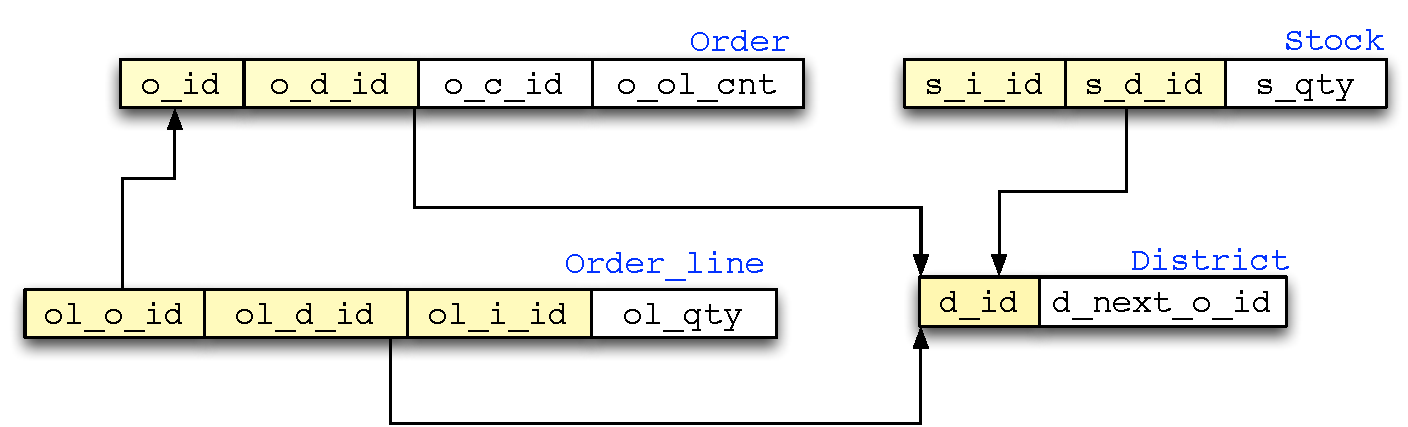
\includegraphics[scale=0.5]{Figures/schema}
% \caption{Database schema of TPC-C's order management system.
%   Columns against highlighted background are primary keys. Arrows denote
%   foreign key relationships.}
% \label{fig:schema}
% \end{figure}

\begin{figure}[t]
  \centering
	\begin{subfigure}{0.48\textwidth}
		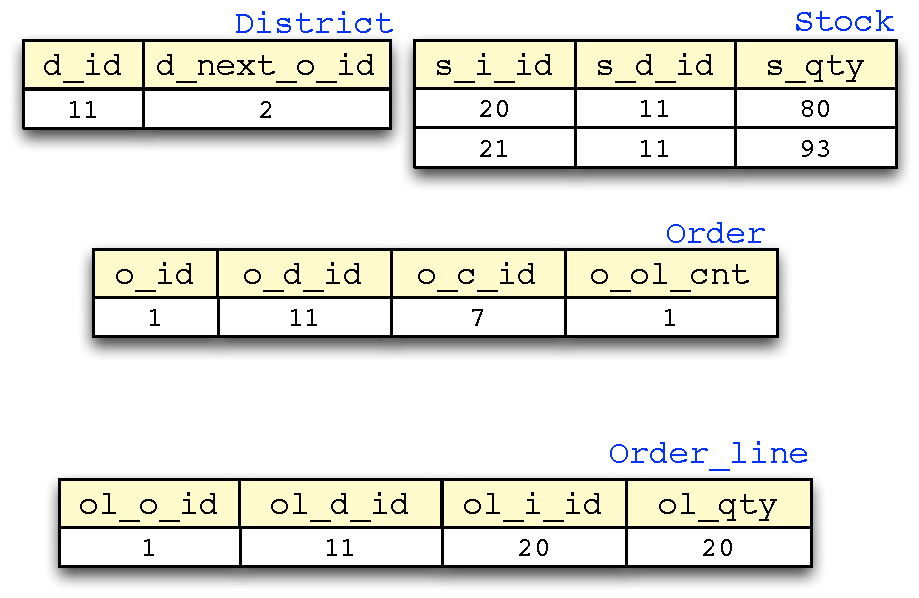
\includegraphics[width=0.9\textwidth]{Figures/schema1}
    \caption{A valid TPC-C database. The only existing order belongs
      to the district with \C{d\_id}=11. It's id (\C{o\_id}) is one
      less than the district's \C{d\_next\_o\_id}, and it's order
      count (\C{o\_ol\_cnt}) is equal to the number of order line
      records whose \C{ol\_o\_id} is equal to the order's id.  }
		\label{fig:tpcc_db1}
	\end{subfigure}
	\begin{subfigure}{0.48\textwidth}
		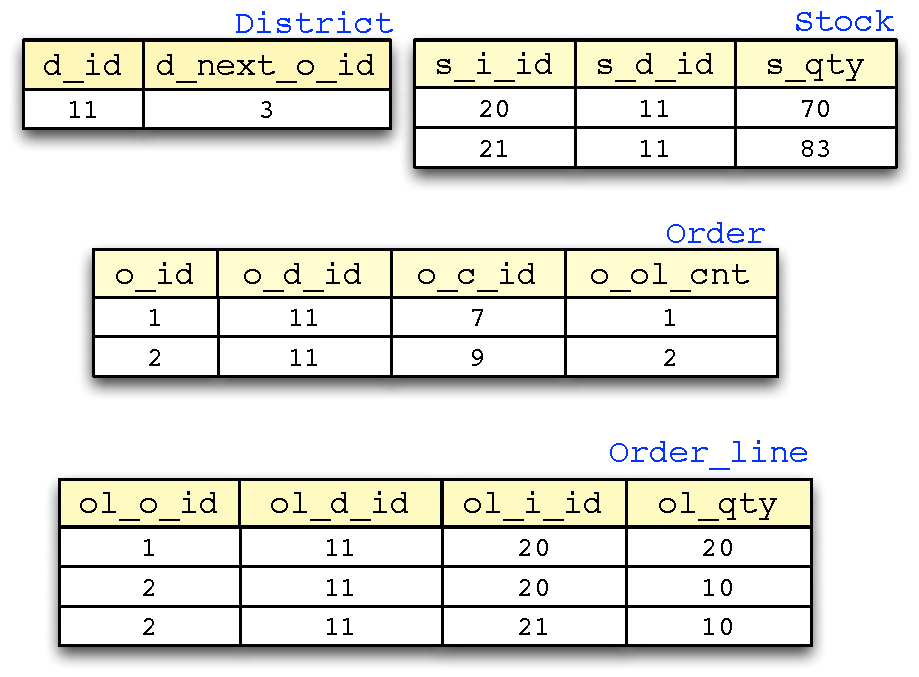
\includegraphics[width=0.9\textwidth]{Figures/schema2}
    \caption{The database in Fig.~\ref{fig:tpcc_db1} after correctly
      executing a \C{new\_order} transaction. A new order record is
      added whose \C{o\_id} is equal to the \C{d\_next\_o\_id} from
      Fig.~\ref{fig:tpcc_db1}. The district's \C{d\_next\_o\_id} is
      incremented. The order's \C{o\_ol\_cnt} is 2, reflecting the
      actual number of order line records whose \C{ol\_o\_id} is equal
      to the order's id (2).}
		\label{fig:tpcc_db2}
	\end{subfigure}

\caption{Database schema of TPC-C's order management system.
  The naming
  convention indicates primary keys and foreign keys. For e.g.,
  \C{ol\_id} is the primary key column of the order line table,
  whereas \C{ol\_o\_id} is a foreign key that refers to the \C{o\_id}
  column of the order table.}
\label{fig:schema}
\end{figure}

The \C{new\_order} transaction inserts a new \C{Order} record, whose
id is the sequence number of the next order under the given district
(\C{d\_id}). The sequence number is stored in the corresponding
\C{District} record, and updated each time a new order is added to the
system. Since each order may request multiple items (\C{item\_reqs}),
an \C{Order\_line} record is created for each requested item to relate
the order with the item. Each item has a corresponding record in the
\C{Stock} table, which keeps track of the quantity of the item left in
stock (\C{s\_qty}). The quantity is updated by the transaction to
reflect the processing of new orders (if the stock quantity falls below
10, it is automatically replenished by 91).

TPC-C defines multiple invariants, called \emph{consistency
conditions}, over the state of the application in the database. One
such consistency condition is the requirement that for a given order
\C{o}, the \emph{order-line-count} field (\C{o.o\_ol\_cnt}) should
reflect the number of order lines under the order; this is the number
of \C{Order\_line} records whose \C{ol\_o\_id} field is the same as
\C{o.o\_id}.  In a sequential execution, it is easy to see how this
condition is preserved.  A new \C{Order} record is added with its
\C{o\_id} distinct from existing order ids, and its \C{o\_ol\_cnt} is
set to be equal to the size of the \C{item\_reqs} set. The \C{foreach}
loop runs once for each \C{item\_req}, adding a new \C{Order\_line}
record for each requested item, with its \C{ol\_o\_id} field set to
\C{o\_id}. Thus, at the end of the loop, the number of \C{Order\_line}
records in the database, whose \C{ol\_o\_id} is equal to \C{o\_id} is
equal to the size of the \C{item\_req} set, which in turn is equal to
the \C{Order} record's \C{o\_ol\_cnt} field, thus preserving the
consistency condition.

Because the aforementioned reasoning is reasonably simple to perform
manually, verifying the soundess of TPC-C's consistency conditions
would appear to be feasible.  Serializability aids the tractability of
verification by preventing any interference among concurrently
executing transactions while the \C{new\_order} transaction executes.
Under weak isolation\footnote{Weak isolation does not violate
  atomicity as long as the witnessed effects are those of committed
  transactions}, however, interferences of various kinds are
permitted.  Although the verification problem for weakly isolated
transactions would appear to be superficially similar to the
verification of (racy) concurrent programs (e.g., garbage
collectors~\cite{JLP+14,GHE15,HPQ+15}), weak isolation introduces new
challenges arising from the use of transactions, and new opportunities
arising from the fact that the store abstraction used by transactions
is a relational database, not low-level memory.

To illustrate some of these challenges, consider the behavior of the
\C{new\_order} transaction when executed with a \emph{Read Committed}
(RC) isolation level, the default isolation level in 8 of the 18
databases studied in~\ref{bailishotos}.  An RC transaction is
isolated from \emph{dirty writes}, i.e., writes of uncommitted
transactions, but is allowed to witness the writes of concurrent
transactions as soon as they are committed. Thus, with two concurrent
instances of the \C{new\_order} transaction (call them $T_1$ and
$T_2$), both concurrently placing new orders for different customers
under the same district (\C{d\_id}), RC isolation allows the
execution shown in Fig.~\ref{fig:new_order_execs}.

\begin{figure}[!t]
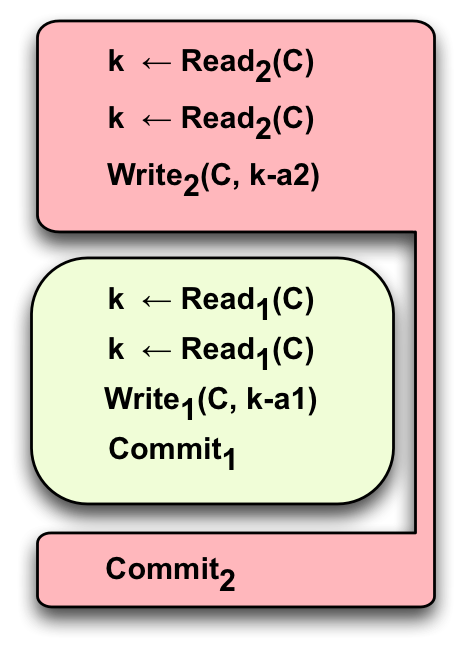
\includegraphics[scale=0.45]{Figures/motiv-eg-1-b}
\caption{\small An RC execution involving two instances ($T_1$ and
  $T_2$) of the \C{new\_order} transaction depicted in
  Fig.~\ref{fig:new_order_code}. 
  Both instances read the \C{d\_id} \C{District} record concurrently,
  because neither transaction is committed when the reads are
  executed.  The subsequent operations are effectively sequentialized,
  since $T_2$ commits. Nonetheless, reading the same value for
  \C{d\_next\_o\_id} prompts both instances to add \C{Order} records
  with same ids, which inturn triggers the the violation of TPC-C's
  consistency condition.}
\label{fig:new_order_exec}
\end{figure}

% \begin{figure}[!h]
% \centering
% \subcaptionbox {
%   {\sc rc} Execution 1
%   \label{fig:motiv-eg-1-b}
% } [
%   0.55\columnwidth
% ] {
%   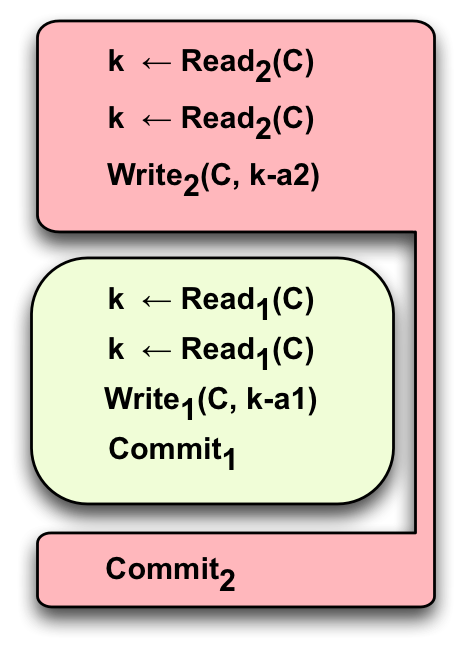
\includegraphics[scale=0.45]{Figures/motiv-eg-1-b}
% }
% %\hspace*{0.5in}
% \subcaptionbox {
%   {\sc rc} Execution 2
%   \label{fig:motiv-eg-1-a}
% }{
%   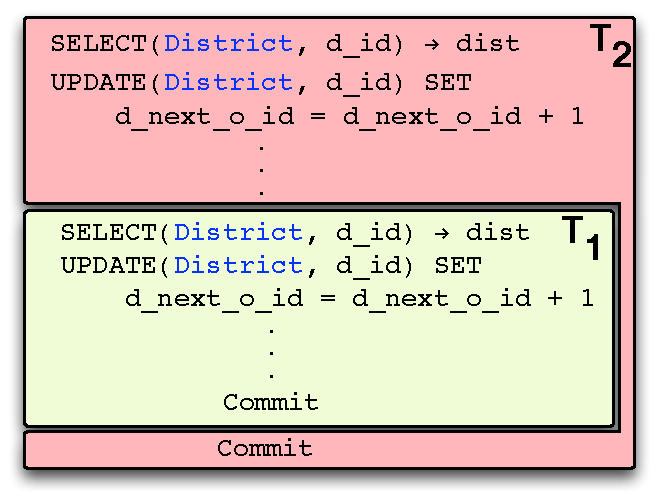
\includegraphics[scale=0.45]{Figures/motiv-eg-1-a}
% }
%   \caption{\small RC executions involving two instances ($T_1$ and
%   $T_2$) of the \C{new\_order} transaction depicted in
%   Fig.~\ref{fig:new_order_code}. 
%   Each instance reads the \C{d\_id} \C{District} record twice, the second
%   time to (atomically) update the \C{d\_next\_o\_id} field.}
% \label{fig:new_order_execs}
% \end{figure}

The figure depicts an execution as a series of SQL 
operations. In the execution, the \C{new\_order} instance
$T_1$ (green) reads the \C{d\_next\_o\_id} field of the district
record for \C{d\_id}, but before it increments the field, another
\C{new\_order} instance ($T_2$) begins its execution and commits. Note
that $T_2$ reads the same \C{d\_next\_o\_id} value as $T_1$, and
inserts new \C{Order} and \C{Order\_line} records with their \C{o\_id}
and \C{ol\_o\_id} fields (resp.) equal to \C{d\_next\_o\_id}. $T_2$
also increments the \C{d\_next\_o\_id} field, which $T_1$ has already
acccessed. This is allowed because reads do not obtain a mutually
exclusive lock on most databases. After $T_2$'s commit, $T_1$ resumes
execution and adds new \C{Order} and \C{Order\_line} fields with the
same order id as $T_1$. Thus, by the end of the execution,
\C{Order\_line} records inserted by $T_1$ and $T_2$ all bear the same
order id. There are also two \C{Order} records with the same district
id (\C{d\_id}) and order id, none of whose \C{o\_ol\_cnt} reflects the
actual number of \C{Order\_line} records inserted with that order id.
This clearly violates TPC-C's consistency condition. 

Notably, this example does not exhibit any of the anomalies that
characterize RC isolation~\cite{berenson}. For instance, there are no
\emph{lost writes}; both concurrent transactions' writes are present
in the final state of the database. Thus, program analyses that aim to
determine appropriate isolation by checking for possible
manifestations of these anomalies would fail to identify grounds for
promoting the isolation level of \C{new\_order} to something stronger.
Yet, if we take the semantics of the application into account, it is
quite clear that RC is not an appropriate isolation level for
\C{new\_order}.

While reasoning in terms of anomalies is cumbersome and inadequate,
reasoning about weak isolation in terms of low-level
traces~\cite{adyaphd,gotsmanconcur15} on memory read and write actions
complicates high-level reasoning.  A possible alternative would
interleave weak isolation implementation details within the program,
yielding a (more-or-less) conventional concurrent program that can be
then subject to classical concurrent verification methods.
Considering the size and complexity of real-world transaction systems,
this strategy is unlikely to scale.

In this paper, we adopt a different approach that \emph{lifts}
isolation semantics (\emph{not} their implementations) to the
application layer, providing a principled framework to simultaneously
reason about application invariants and isolation properties.  To
illustrate this idea informally, consider how we might verify that
\C{new\_order} is sound when executed under \emph{Snapshot Isolation}
(SI), and isolation level stronger than RC. Snapshot isolation
allows transactions to be executed against their respective private
snapshots of the database, thus admitting concurrency, but it also
requires that there not be any write-writeconflicts among
concurrent transactions. Write-write conflicts can be eliminated in various
ways; either through detection followed by a rollback, or through
exclusive locks, or a combination of both, leading to different ways
in which SI can be realized. For instance, one possible implementation
of SI, close to the one use by PostgreSQL~\cite{postgres-ssi},
executes a transaction against its private snapshot of the database,
but obtains exclusive locks on the actual records in the database
before performing writes. A write is performed only if the record
hasn't already been updated by a concurrent transaction, i.e,  when it
doesn't result in a write-write conflict.  Otherwise, the transaction is
rolledback. This implementation is demonstrated for a simple database
with three records, $a$, $b$, and $c$ in Fig.~\ref{fig:RR-postgres}.

\begin{figure}[t]
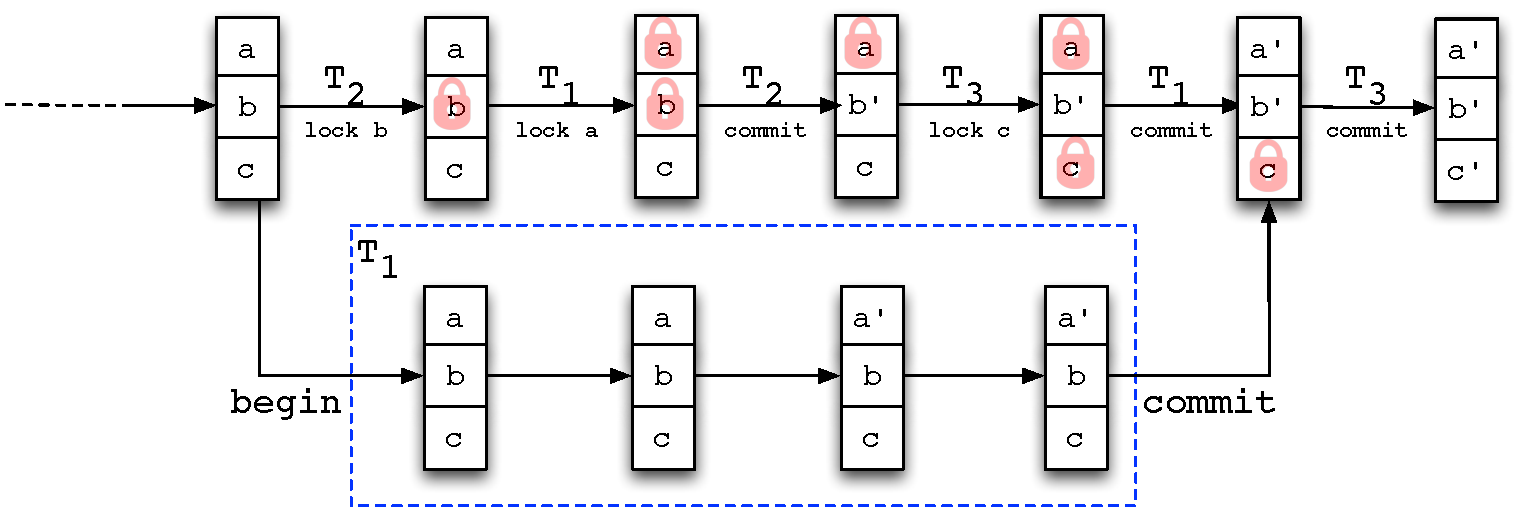
\includegraphics[scale=0.5]{Figures/RR-postgres}
\caption{Database state transitions corresponding to an execution of
  an SI transaction $T_1$ on a PostgreSQL-like store. $T_2$ and $T_3$
  are concurrent transactions. }
\label{fig:rr-postgres}
\end{figure}
\begin{figure}[t]
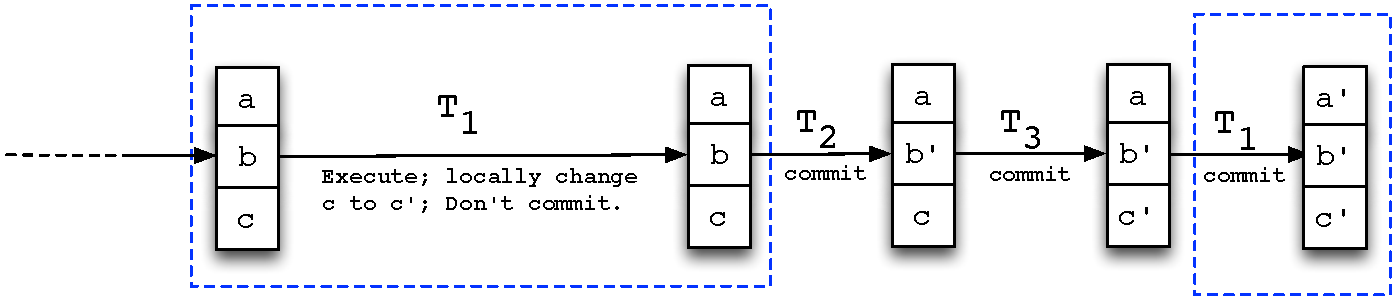
\includegraphics[scale=0.5]{Figures/RR-abstract}
  \caption{An abstract execution that includes the concrete execution
  shown in Fig.~\ref{fig:rr-postgres}. It has no locks or snapshots,
  admits fewer interleavings, yet results in the same post-state.  }
\label{fig:rr-abstract}
\end{figure}

Implementations of SI on real databases (e.g., PostgreSQL) are
complicated, often running into thousands of lines of code.
Nonetheless, the semantics of Snapshot Isolation, in terms of how it
effects the transitions on the database state, can be captured in a
fairly simple model. Firstly, although SI admits concurrent
transactions, their effects are  not witnessed in the current
transaction (call it $T$), during $T$'s execution. Thus, insofar as
$T$ is concerned, the global state doesn't change as long as it
executes. More formally, for every consecutive pair of global states
$(\stg,\stg')$ witnessed by $T$ during its execution, SI requires
$\stg'=\stg$.  After $T$ finishes execution, it commits to the actual
database, which incorporates the effects of concurrent transactions.
In executions where $T$ successfully commits, concurrent transactions
are guaranteed to not be in write-write conflict with $T$. Thus, if
$\stg$ is the global state that $T$ witnessed when it finished
execution (which would be same as the snapshot state), and $\stg'$ is
the state to which $T$ commits, then the diff between $\stg$ and
$\stg'$ shouldn't be in a write-write conflict with $T$. To concretize
this notion, let the database state be a map from transaction
variables to values, and let $\stl$ denote a transaction-local log
that maps the variables being written to their updated values. Then
the absence of write-write conflicts between $T$ and the diff between
$\stg$ and $\stg'$ can be defined as: $\forall
x\in\mathit{dom}(\delta)$, $\stg'(x) = \stg(x)$.  To summarize, the
semantics of SI can be captured as an axiomatization over transitions
of the database state ($\Delta \longrightarrow \Delta'$) during the
lifetime an SI transaction ($T$):
\begin{itemize}
  \item While $T$ executes, $\Delta' = \Delta$.
  \item After $T$ finishes execution, but before it commits its local
    state $\delta$, $\forall(x\in\delta).~\Delta'(x) = \Delta(x)$.
\end{itemize}

% nor $T$'s effects are
% witnessed by concurrent transactions, during $T$'s execution. Thus,
% $T$'s execution can be thought of as a series of transitions of a
% state local to $T$ (call it $\stl$), that has no bearing outside $T$. Conversely, any
% transitions performed by the concurrent transactions on the global
% state (call it $\stg$) has no
% bearing on $T$ since $T$ reads off a static snapshot established at
% the beginning of the transaction. Consequently, any
% state transitions performed by the concurrent transactions can be
% \emph{moved past} $T$'s local state transitions. $T$'s commit,
% however, is a global state transition that is enabled only if
% there are no WW conflicts between $T$ and concurrent transactions.
% Thus, concurrent transactions' state transitions cannot be moved past
% $T$'s commit, and $T$ can be thought of witnessing the effects of
% concurrent transactions just before its commit. 
% therefore treat Since a
% transaction's reads are always served from a snapshot, no state
% changes are witnessed while the execution is in progress. Thus,
% insofar as an RR transaction is concerned, the database state does not
% change during the execution.  Uncommitted writes are recorded in a
% transaction-local state.  When the transaction commits, the local
% state is atomically written to the global state to yield a global
% state that reflects the transaction's updates.  However, unlike a
% strongly isolated serializable transaction, the commit operation is
% performed against the current state of the database, not the
% snapshot. Thus, after the transaction finishes execution, but before
% it commits, the transaction is able to witness the effects of all
% concurrent transactions that committed before it.  The PostgreSQL RR
% implementation effectively constrains this transition.

% We can axiomatize this operational description by observing that (a)
% due to the version check, the current transaction cannot update a data
% item that was already updated by a concurrent transaction, and (b) due
% to the use of exclusive write locks, a data item updated by the
% current transaction cannot be overwritten by a concurrent transaction.
% If $\Delta$ is the state of the database when an RR transaction
% finishes, and $\Delta_c$ is the state visible to the transaction at
% the point of commit, we know the transition from $\Delta$ to
% $\Delta_c$ (written $\Delta \longrightarrow \Delta_c$) cannot exhibit
% effects from any concurrent transactions that write to the same data
% items as the current RR transaction.  Similarly, if $\delta$ denotes
% a local log that relates transaction variables being written with their updated values,
% then $\forall x\in\mathit{dom}(\delta)$, $\Delta_c(x) =
% \Delta(x)$. To summarize, the operational semantics of PostgreSQL's RR
% implementation can be captured as an axiomatization over transitions of
% the database state ($\Delta \longrightarrow \Delta'$) during the
% lifetime an RR transaction ($T$):
% \begin{itemize}
%   \item While $T$ executes, $\Delta' = \Delta$.
%   \item After $T$ finishes execution, but before it commits its local
%     state $\delta$, $\forall(x\in\delta).~\Delta'(x) = \Delta(x)$.
% \end{itemize}

This simple characterization of SI isolation allows us to verify the
consistency conditions associated with the \C{new\_order} transaction.
First, since the database doesn't change ($\Delta' = \Delta$) during
the execution of the transaction's body, we can reason about
\C{new\_order} as though it executed in complete isolation until its
commit point, leading to a verification process similar to what would
been applied when reasoning about serializability.  When
\C{new\_order} finishes execution, but before it commits, the SI
axiomatization shown above requires us to consider global state
transitions $\stg \longrightarrow \stg'$ that do not include changes
to the records ($\stl$) written by \C{new\_order}, i.e.,
$\forall(x\in\delta).~\Delta'(x) = \Delta(x)$. Since concurrent
\C{new\_order} transactions that write to the same \C{District} record
modify the record by incrementing its \C{d\_next\_o\_id} field, their
transitions do not satisfy the necessary condition imposed by the SI
axiomatization, allowing us to rightfully ignore their interference.
This leaves the interference due to concurrent \C{new\_order}
transactions that write to a different district record.  Fortunately,
such interference does not prompt \C{new\_order} to violate the
invariant, which can be established by adopting a reasoning similar to
the one used on concurrent program logics, such as the Rely-Guarantee
logic, customized for the database programs. Our approach generalizes
this style of reasoning to a range of isolation levels, concurrency
control techniques, and their combinations used frequently in practice.

% and becomes ready to commit, a
% transition transfers the transaction's local writes ($\delta$) to the
% unchanged database state ($\Delta$).  However, we are required to
% consider the interference from concurrent transitions at this point,
% which might change the database state from $\Delta$ to $\Delta_c$. If
% this interference includes the effects of a concurrent \C{new\_order}
% transaction (with the same \C{d\_id}), then verification fails as
% described previously.  Fortunately, sequential reasoning shows that
% this is impossible - RR prevents a concurrent \C{new\_order}
% transaction that modifies the same \C{District} record as the current
% transaction (concretely, since the record is already present in the
% current transaction's local log, any transition from $\Delta$ to
% $\Delta_c$ cannot change this record).  Applying such axiomatic
% reasoning on \C{new\_order} allows us to prove that the TPC-C
% invariant holds when the transaction is executed under PostgreSQL's RR
% isolation.  Our proof framework generalizes this style of reasoning to
% various isolation levels on databases.

The second observation that informs our approach is one that pertains
to automation. Program verification, even when machine-aided, often
entails significant annotation burden in the form of intermediary
assertions and loop invariants required to prove a program correct.
This is certainly true for concurrent program logics, such as
Rely-Gurantee, which extend Hoare logic with additional artifacts and
where (stable) intermediary assertions and loop invariants remain a
major source of annotation burden.  However, a relational database is
a significantly simpler abstraction than shared memory. There are no
pointers, linked data structures, or aliasing.  Although a database
essentially abstracts a mutable state, the state is mutated through a
well-defined fixed number of interfaces (SQL statements), each tagged
with a logical formula describing what records are accessed and
updated.

This observation leads us away from thinking of database transactions
as concurrent imperative programs.  Instead, we see value in viewing
them as essentially functional computations that manage database state
monadically. We find it useful to reason about
statements that mutate the database state, not in terms of a pre- and
post-condition pair, but in terms of a state transformer that relates
the pre- and post-states of a statement. This state transformer
semantics can be defined algorithmically, just like predicate
transformer semantics (e.g., strongest post-condition).  Here, a state
transformer interprets a SQL statement in the set domain, taking
advantage of the fact that the database is essentially a set of
tuples, and a SQL statement is a transformer over these sets.  The
benefit of this approach is that low-level loops can now be
substituted with higher-order combinators that automatically lift the
state transformer of its higher-order argument (i.e., the loop body)
to the state transformer of the combined expression (i.e., the loop).
Thus the semantics of a \C{foreach} loop, for instance, can be
captured as a state transformer, where the state is a set, and the
transformation defines a bind operation. We illustrate this intuition
on a simple example.

% \begin{figure}[!t]
% \centering
% %
% \begin{subfigure}[b]{0.46\textwidth}
% \begin{ocaml}
% Set s' = $\emptyset$;
% foreach x in s {
%   s'.add(f(x)); 
% }
% \end{ocaml}
% \caption{}
% \end{subfigure}
% %
% \begin{subfigure}[b]{0.5\textwidth}
% \begin{ocaml}
% let s' = ref [];
% foreach s (fun x -> s' := x::(!s'));
% \end{ocaml}
% \caption{Lorem ipsum, lorem ipsum,Lorem ipsum, lorem ipsum,Lorem ipsum}
% \end{subfigure}
% \caption{Caption place holder}
% %
% \caption{New versions are created from existing versions either
% through \C{push} or \C{merge}.}
% \label{fig:syntactic-ancestors}
% \end{figure}
% let s' = ref (Set.empty) in
% foreach xs @@ fun x -> 
%   begin
%     s' := Set.union !s' @@ 
%             Set.map_selected s (fun y -> y<x)
%                                (fun y -> y+x);
%     s' := Set.add !s' x;
%   end
\begin{figure}[!h]
\begin{ocaml}
foreach item_reqs @@ fun item_req -> do
  SQL.update Stock (fun s -> {s with s_qty = k1}) 
                   (fun s -> s.s_i_id = item_req.ol_i_id);
  SQL.insert Order_line {ol_o_id=k2; ol_d_id=k3; 
                         ol_i_id=item_req.ol_i_id; ol_qty=item_req.ol_qty}
\end{ocaml}
\caption{Foreach loop from Fig.~\ref{fig:new_order_code}}
\label{fig:foreach_code}
\end{figure}

Fig.~\ref{fig:foreach_code} shows a (simplified) snippet of code taken
from Fig.~\ref{fig:new_order_code}. Some irrelevant expressions have
been replaced with constants (\C{k1} to \C{k3}).  The body of the loop
executes a SQL update followed by an insert.  Recall that a transaction
reads from the global database ($\Delta$), and writes to a
transaction-local database ($\delta$) before committing these updates. An update
statement filters the tuples that match the search criteria from $\Delta$
and computes the updated tuples that are to be
added to the local database. Thus, its state transformer (call it
$\T_U$) is the following function on sets\footnote{$\bind$ has higher
precedence than $\cup$.}:
\begin{smathpar}
\begin{array}{l}
  \lambda(\stl,\stg).~ \stl \cup \stg \bind(\lambda s. 
      \itel{{\sf table}(s) = \C{Stock} \conj 
                s.\C{s\_i\_id} = \C{item\_req.ol\_i\_id}\\\hspace*{1.3in}} 
           {\{\{s \with \C{s\_qty} = \C{k1}\}\}\\\hspace*{1.3in}}
           {\emptyset}
\end{array}
\end{smathpar}
% \begin{smathpar}
% \begin{array}{c}
%   \lambda\Delta.\lambda\delta.\, \delta \;\cup\; 
%       \Delta \,\bind\, (\lambda s.\, 
%           \C{if}\;{\C{stock}(s) \conj 
%                    \C{s.s\_i\_id} = \C{item\_req.ol\_i\_id}}\\
%            \hspace*{0.9in}
%            \C{then}\;{\{\{s \;\C{with}\; \C{s\_qty} = \C{k1}\}\}}\;
%            \C{else}\;{\emptyset})
% \end{array}
% \end{smathpar}
% \begin{verbatim}
%   Rmem(σ'(s')) = Rmem(σ(s')) U 
%                  Rmem[\x. Rmem[\y. if y<x then {y+x} else {}](σ(s)) U {x}](xs)
% \end{verbatim}
% Observe that
% $\T_U(\Delta,\delta)$ is of the form $\delta \,\cup\,
% F_U(\Delta)$. 
The transformer ($\T_I(\Delta,\delta)$) for the subsequent \C{insert}
statement can be similarly calculated as the following:
\begin{smathpar}
\begin{array}{l}
  \lambda(\stl,\stg).~ \stl \cup \{\C{ol\_o\_id}=\C{k2};\, 
        \C{ol\_d\_id}=\C{k3};\, \C{ol\_i\_id}=\C{item\_req.ol\_i\_id};\, 
        \C{ol\_qty}=\C{item\_req.ol\_qty}\}
\end{array}
\end{smathpar}
Observe that both transformers are of the form $T(\Delta,\delta) =
\stl \cup F(\stg)$, where $F$ is a function that returns the set of
records added by the transformer to the transaction-local database
($\stl$). Let $\F_U$ and $\F_I$ be the corresponding functions for $\T_U$
and $\T_I$ shown above. The state transformed of the loop body in
Fig.~\ref{fig:new} can be expressed as the following composition of
$\F_U$ and $\F_I$:
\begin{smathpar}
\begin{array}{l}
  \lambda(\stl,\stg).~ \stl \cup \F_U(\stg) \cup \F_I(\stg)
\end{array}
\end{smathpar}
The transformer for the loop itself can now be computed as following:
\begin{smathpar}
\begin{array}{l}
  \lambda(\stl,\stg).~ \stl \cup \C{item\_reqs}\bind
      (\lambda\C{item\_req}.~ \F_U(\stg) \cup \F_I(\stg))
\end{array}
\end{smathpar}
Observe that the structure of the transformer mirrors the structure of
the program itself. In particular, SQL statements become set
operations, and the \C{DB} monad's $\bind$ becoms set monadic $\bind$.
Thus, state transformer inference is completely mechanical. The
advantage of inferring such transformers is that we can now make use
of a semantics-preserving translation from the domain of sets equipped
with $\bind$ to the first-order logic, allowing us to leverage SMT
solvers for automatic proofs without having to infer loop invariants,
or provide intermediate assertions.  Sec.~\ref{sec:inference}
describes this translation. In the exposition thus far, we assumed
$\Delta$ remains invaraint, which is clearly not the case when we
admit concurrency.  Necessary concurrency extensions of the state
transformer semantics is also covered in Sec.~\ref{sec:inference}.
The following two sections, however, first focus on laying the
theoretical foundations for reasoning about weak isolation.
